\documentclass[letterpaper,12pt]{article}
\usepackage{tabularx} % extra features for tabular environment
\usepackage{amsmath}  % improve math presentation
\usepackage{float}
\usepackage{pdfpages}


\usepackage{graphicx} % takes care of graphic including machinery
\graphicspath{ {./figures/} }
%\usepackage[margin=1in,letterpaper]{geometry} % decreases margins
%\usepackage{cite} % takes care of citations
\usepackage[final]{hyperref} % adds hyper links inside the generated pdf file
\hypersetup{
	colorlinks=true,       % false: boxed links; true: colored links
	linkcolor=blue,        % color of internal links
	citecolor=blue,        % color of links to bibliography
	filecolor=magenta,     % color of file links
	urlcolor =blue         
}
\usepackage[margin = 1in,headsep=0.5cm,headheight=2cm,letterpaper]{geometry} 

\usepackage{fancyhdr}
\pagestyle{fancy}
\lhead{Student 1 : Ahmet Akman 2442366 \\ Student 2: Yusuf Toprak Yıldıran 2444149 \\ Assistant: Onur Selim Kılıç}
\rhead{Date: \today \\ Group: Wednesday Morning - 5} 
%\cfoot{center of the footer!}
\renewcommand{\headrulewidth}{0.1pt}
%

%\renewcommand{\footrulewidth}{0.4pt}



\begin{document}
\thispagestyle{empty}

\title{Spring 2022 EE214 Experiment 1  \protect\\ Diodes and Rectifiers}
\author{Ahmet Akman 2442366 \protect\\ Yusuf Toprak Yıldıran 2444149 \protect\\ Assistant: Onur Selim Kılıç}
\date{\today}
\maketitle
\tableofcontents
%\begin{abstract}
%abstract
%\end{abstract}
\section{Introduction}
In this experiment, the characteristics of different diodes and rectifiers are investigated. First, the i-v characteristics of 3 different diodes are expected to be observed. Then, the behavior of the half-wave rectifier is expected to be experimented with. Lastly, observations are made on clamper and regulator with zener diode circuits. The results of the experimentation are evaluated and reported in this document.
\section{Experimental Results and Discussion}
The results of the experiment are discussed in the following steps.
\subsection{Step 1}
In this step, the circuit schematic given in Figure 1 is constructed on the breadboard. The analog signal generator is used for floating output as the signal supply.
\begin{figure}[H]
\centering
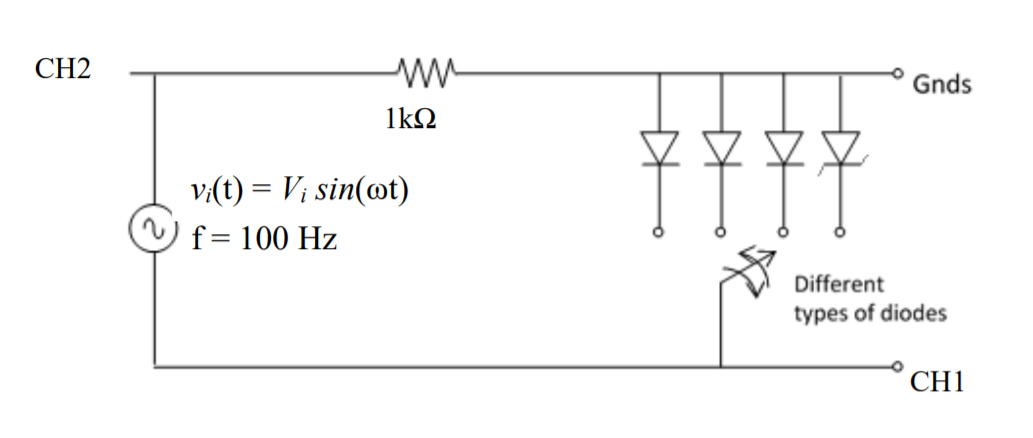
\includegraphics[width = 0.75\textwidth]{1_1.png}
\caption{Circuit schematic for step 1}
\end{figure} 

\subsubsection{a)}
%\href{https://www.vishay.com/docs/88503/1n4001.pdf}{1N40007} 
The diode models, \href{https://logosfoundation.org/elektron/mixers/AA119.pdf}{AA119},\href{https://www.vishay.com/docs/88536/ba157.pdf}{BA159}  ,and \href{https://www.vishay.com/docs/85604/bzx55.pdf}{BZX55C-6V2} are used. The probes of the oscilloscope is connected to the nodes indicated in Figure 1. The resulting graph is plotted as given in Figure 2 , 3 ,and 4 for \href{https://logosfoundation.org/elektron/mixers/AA119.pdf}{AA119},\href{https://www.vishay.com/docs/88536/ba157.pdf}{BA159}  ,and \href{https://www.vishay.com/docs/85604/bzx55.pdf}{BZX55C-6V2} respectively.

\begin{figure}[H]
    \centering
    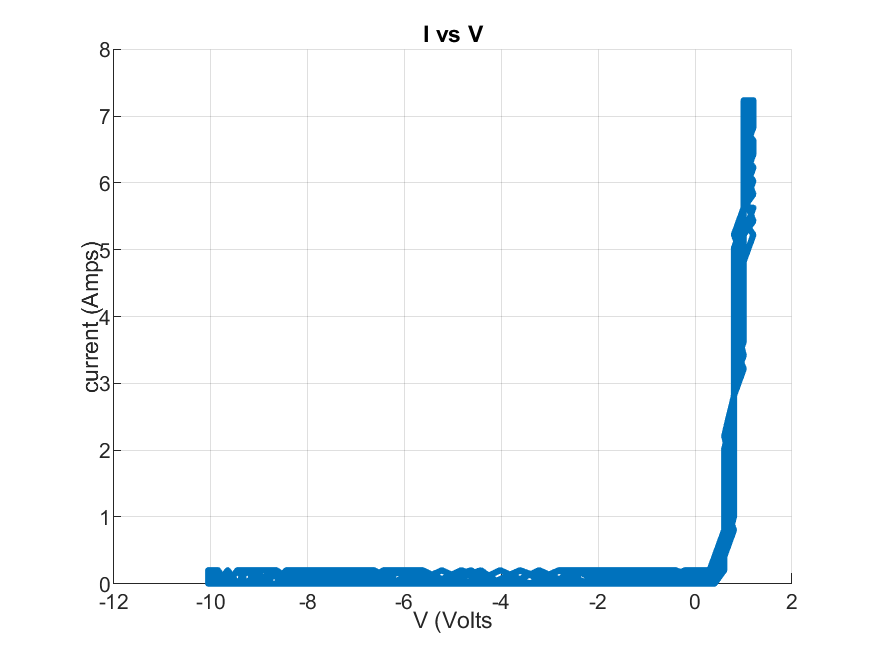
\includegraphics[width = 0.75\textwidth]{1_aa119.png}
    \caption{i-v characteristics of AA119}
\end{figure} 


\begin{figure}[H]
    \centering
    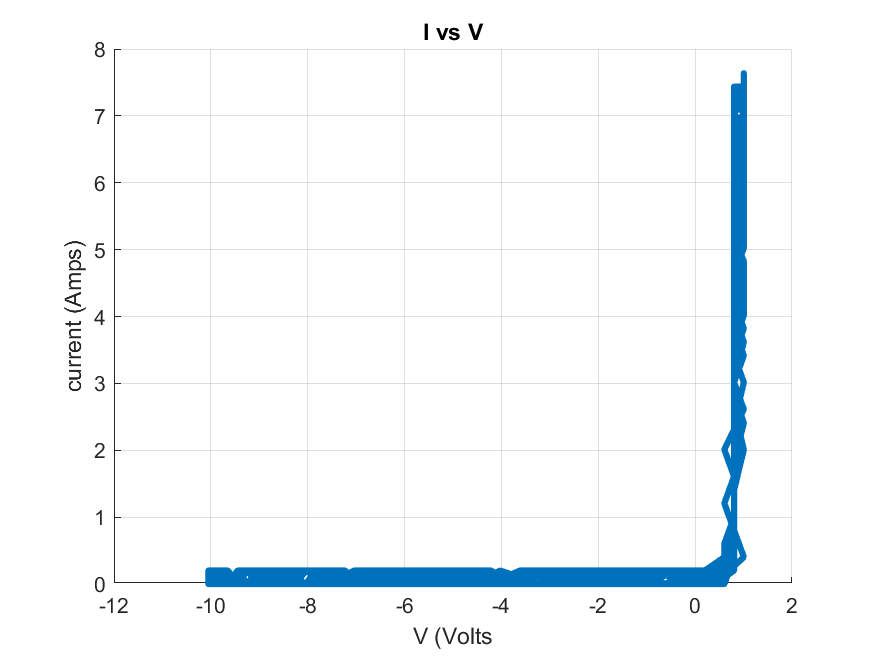
\includegraphics[width = 0.75\textwidth]{1_ba159.png}
    \caption{i-v characteristics of BA159}
\end{figure} 


\begin{figure}[H]
    \centering
    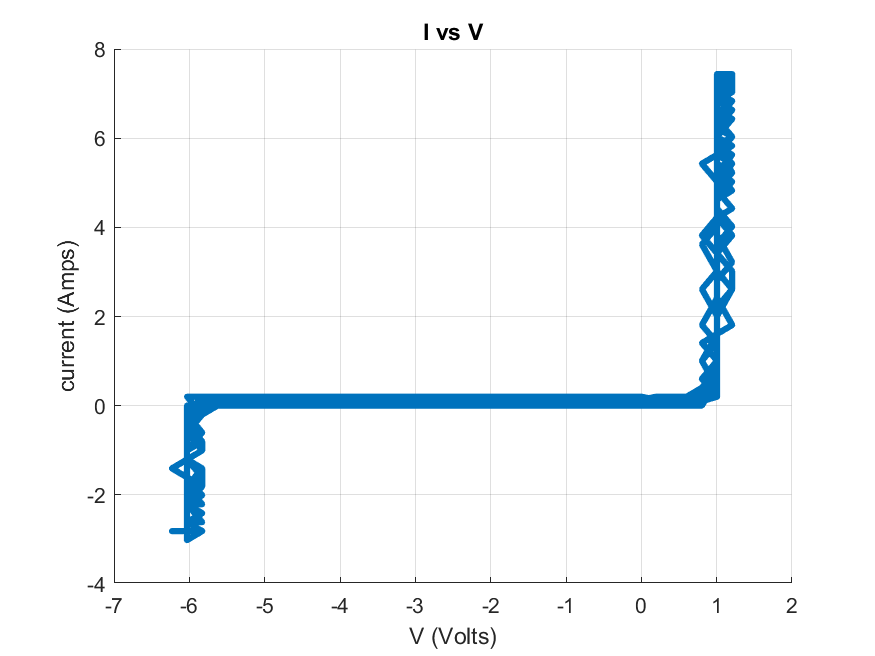
\includegraphics[width = 0.75\textwidth]{1_zener.png}
    \caption{i-v characteristics of BZX55C-6V2}
\end{figure} 


Using those plots, the piecewise parameters of the diodes are obtained by virtue of the cursors of the oscilloscope. The parameters of diode AA119 are given in Table 1.

\begin{table}[H]
    \begin{center}
    \caption{Piecewise parameters of diode AA119}
    \vspace{2mm}
    \begin{tabular}{|| c | c | c ||}
    \hline
    \(V_{on}\) & 350 mV \\
    \hline 
    \(r_f\) & 0.17 \(\Omega\) \\
    \hline
    \(r_r\) & 86 \(\Omega\)\\
    \hline
    \end{tabular}
\end{center}
\end{table}
The obtained parameters of diode AA119 are given in Table 2.
\begin{table}[H]
    \centering
    \caption{Piecewise parameters of diode BA159}
    \vspace{2mm}
    \begin{tabular}{||c | c | c||}
    \hline
    \(V_{on}\) & 973.5 mV \\
    \hline
    \(r_f\) & 0.625 \(\Omega\) \\
    \hline
    \(r_r\) & 86.2 \(\Omega\)\\
    \hline
    \end{tabular}
\end{table}
The obtained parameters of diode BZX55C-6V2 are given in Table 3.
\begin{table}[H]
    \centering
    \caption{Piecewise parameters of diode BZX55C-6V2}
    \vspace{2mm}
    \begin{tabular}{||c | c | c||}
        \hline
    \(V_{on}\) & 752 mV \\
    \hline
    \(V_{z}\) & 5.92V \\
    \hline
    \(r_f\) & 0.05 \(\Omega\) \\
    \hline
    \(r_r\) & 0.156 \(\Omega\) \\
    \hline
    \end{tabular}
\end{table}
So, the fundamental i-v characteristics of 3 different diodes are obtained and analyzed using the plot. But, it should be pointed out that the precision of the measurement is quite dependent on the cursor sensitivity of the DSO.

\subsubsection{b)}
In this part, the frequency of the signal generator is adjusted, and the i-v characteristics are observed again. The plot given in Figure 5 is obtained.

\begin{figure}[H]
    \centering
    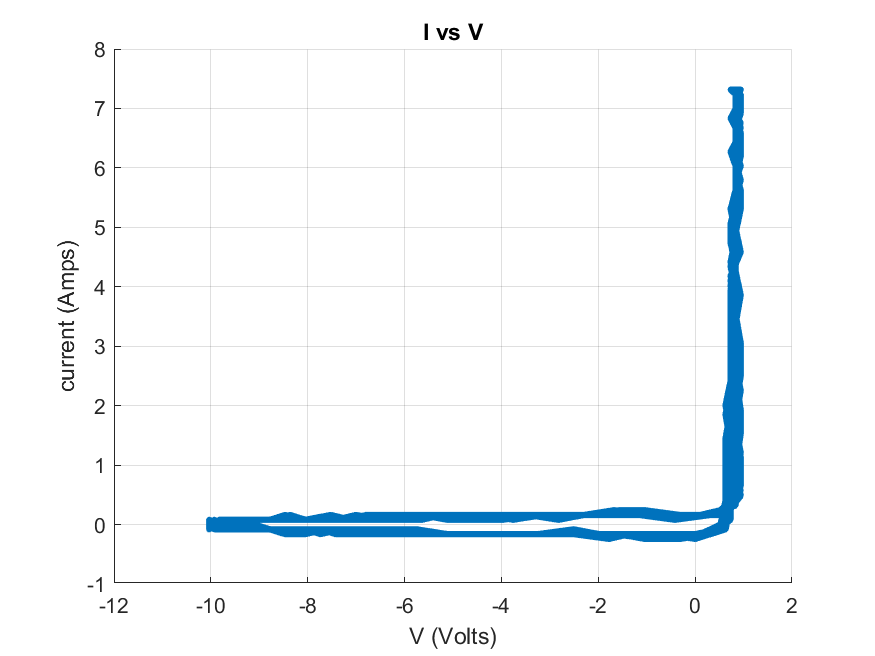
\includegraphics[width = 0.75\textwidth]{1_ba159_10khz.png}
    \caption{i-v characteristics of BA159 at 10khz}
\end{figure} 
It can be said that there is a slight separation on horizontal lines in a plot different than the lower frequency plot. We can call the separation of lines in this i-v graph as hysteresis effect. When we increased the frequency to 10kHz, we observed a hysteresis effect on the i-v characteristics of the diode on the DSO screen. We observe this effect since our diode can not change its state as fast as our high-frequency voltage source supply. To solve this problem and to be able to use diodes at high frequencies, there are "high speed" or "switching" diodes. These diodes can be used in high frequencies without observing the hysteresis effect.

\subsection{Step 2}

\begin{figure}[H]
    \centering
    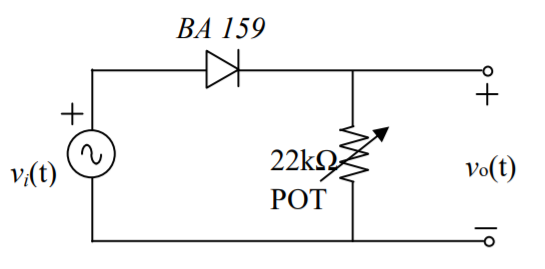
\includegraphics[width = 0.75\textwidth]{2_1.png}
    \caption{Circuit schematic for the step 2}
\end{figure} 
For this part, we set the half-wave rectifier circuit given in Figure 6 and adjusted the signal generator as 
\(
v_i(t)  = 2sin(2000 \pi t) V 
\)


\subsubsection{a)}

POT is set to \(1k\Omega\), and output and input voltage waveforms on the graph indicated in Figure 7 are obtained.

\begin{figure}[H]
    \centering
    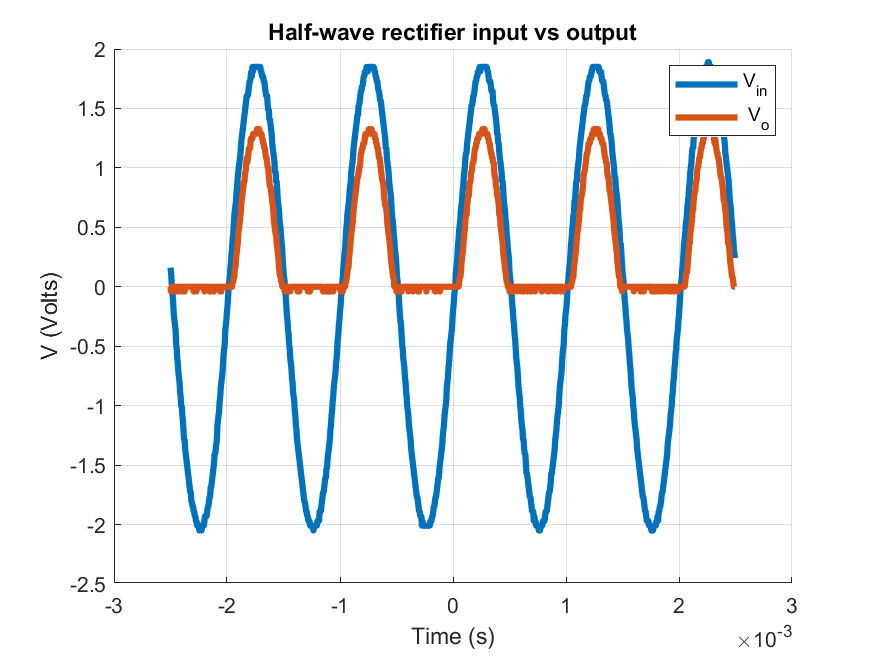
\includegraphics[width = 0.75\textwidth]{2_a.png}
    \caption{Half-wave rectifier with BA159}
\end{figure} 



If one looks at the graph carefully, it can be realized that the output voltage is slightly lower than the input voltage since the diode consumes energy, so it has an internal resistance. Then we measured the \(DC_{rms} \) of output value as 730mV using cursors of DSO. The output voltage waveform on the DSO screen is in a similar shape to the input waveform in positive cycles but zero when input is in the negative cycle.  


\subsubsection{b)}
In this part, in addition to the circuit given in Figure 6, a capacitor of 10\(\mu\)F is connected parallel to the potentiometer. Also the input signal is adjusted to \(10 sin(20 \pi t) \). First, POT is set to \(10k\Omega\), and output and input voltage waveforms on the graph presented in Figure 8 are obtained.

\begin{figure}[H]
    \centering
    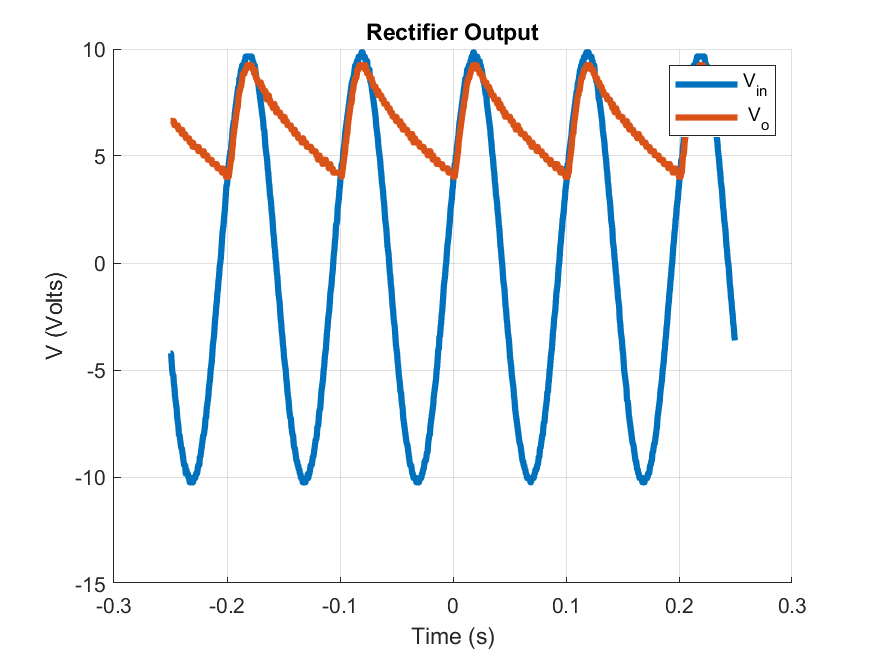
\includegraphics[width = 0.75\textwidth]{2_b_POT_10K.png}
    \caption{Half-wave rectifier with BA159 with pot set to 10K \(\Omega\)}
\end{figure} 
For this plot, it can be said that because of the discharging process of the capacitor, the falling edge of the output signal is different from the case without a capacitor. 
The pot is adjusted to a maximum (18K\(\Omega\)), and the plot given in Figure 9 is obtained.
\begin{figure}[H]
    \centering
    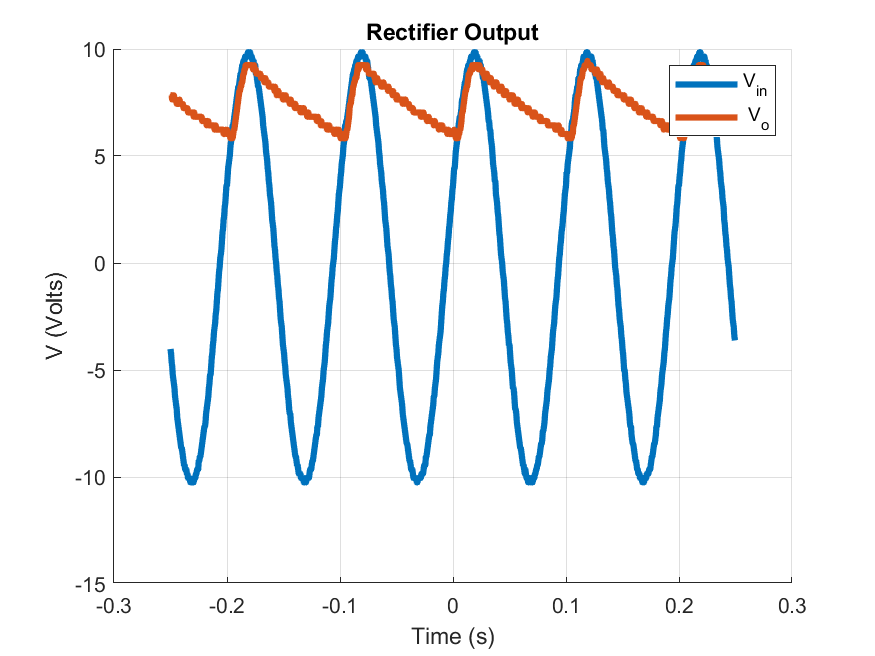
\includegraphics[width = 0.75\textwidth]{2_b_POT_18K.png}
    \caption{Half-wave rectifier with BA159 with pot set to 18K \(\Omega\)}
\end{figure} 
Here it can be said that ripple voltage is decreased as it moved from 10K\(\Omega\).
Lastly, the potentiometer is set to a minimum (1.2K\(\Omega\)). The plot given in Figure 10 is obtained. 

\begin{figure}[H]
    \centering
    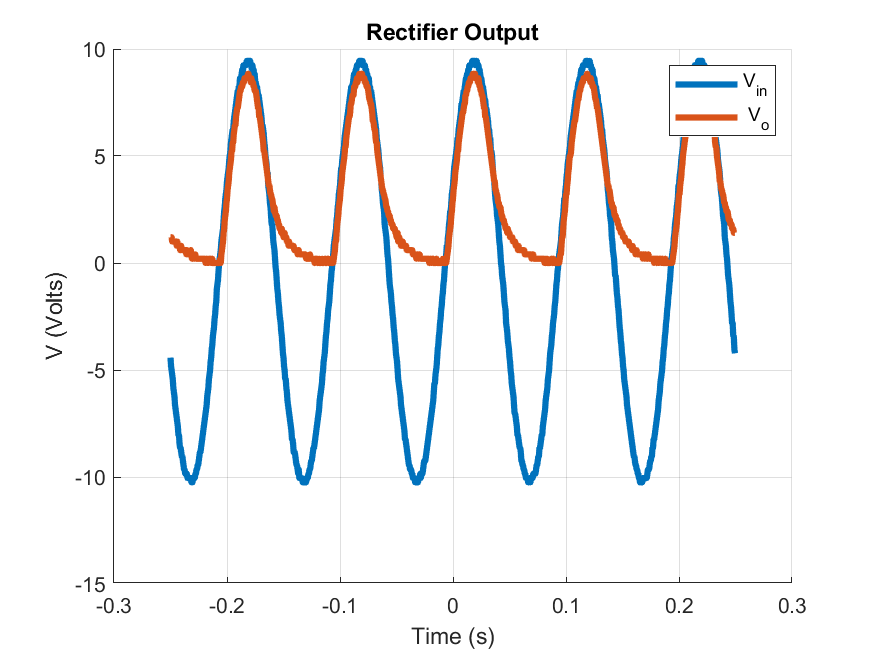
\includegraphics[width = 0.75\textwidth]{2_b_POT_1_2K.png}
    \caption{Half-wave rectifier with BA159 with pot set to 1.2K \(\Omega\)}
\end{figure} 
Here the ripple voltage is higher than in other cases and equal to the case in which the capacitor is absent.

As a result, the \(V_{DC}\), \( V_r \) values are recorded and given in Table 4.

\begin{table}[H]
    \centering
    \caption{Piecewise parameters of diode BZX55C-6V2}
    \vspace{2mm}
    \begin{tabular}{||c | c | c | c||}
        \hline
    R (Ohms)& C (\(mu\) Farads) &\(V_{DC}\) (Volts) & \(V_{r , pp}\) (Volts) \\
    \hline
    10K & 10 & 7.24 & 5.2 \\
    \hline
    18K & 10 & 8.04 & 4.8 \\
    \hline
    1.2K & 10 & 5.03 & 8.8 \\
    \hline
    \end{tabular}
\end{table}
To decrease the ripple voltage in the case of constant resistance, there are three options that can be done. First, the capacitance of the capacitor can be increased so that it would take longer for the resistor to consume its energy. Secondly, if the frequency of the input is increased, the time interval of discharging drops, so ripple voltage may decrease. Lastly, even though it is not feasible, a diode with a higher internal capacitance can be used to decrease ripple voltage.

\subsection{Step 3}

In this third step, we set up the diode clamper circuit given in Figure 11 using the diode 1N4001 and set the voltage \(v_i(t) = 10sin(200\pi t) V\). Then it is plotted the input and output voltage waveforms on the graph given in Figure 12.

\begin{figure}[H]
    \centering
    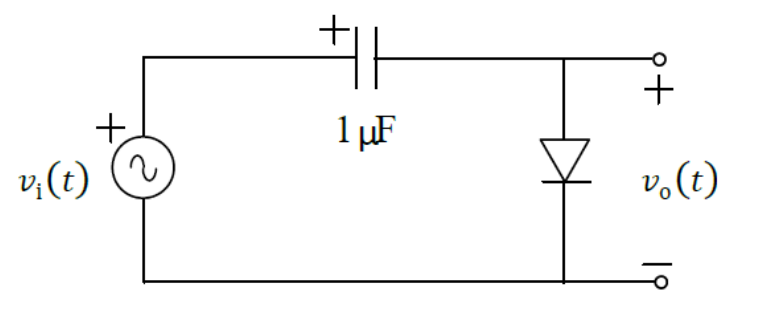
\includegraphics[width = 0.75\textwidth]{3_1.png}
    \caption{Circuit schematic for the step 3}
\end{figure} 
    

\begin{figure}[H]
    \centering
    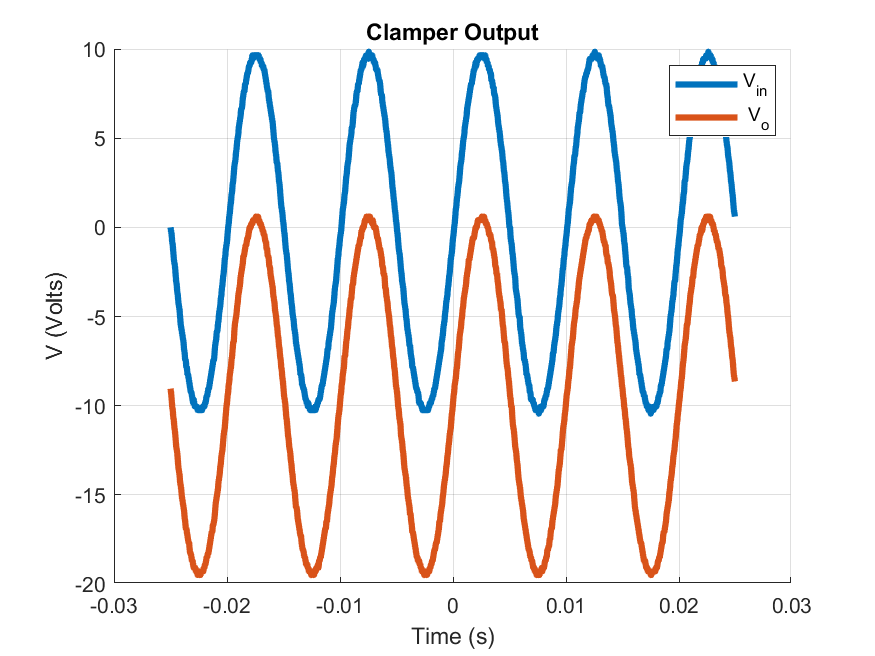
\includegraphics[width = 0.75\textwidth]{3.png}
    \caption{Clamper circuit output }
\end{figure} 
    
From the above graph, we can derive that the output waveform is slightly shifted from of input waveform to below zero. Since the diode prevents the capacitor from being discharged, the peak value of output to be clamped above zero diodes should go into negative bias.



\subsection{Step 4}

In this last part, we set the circuit given in Figure 13 with the load resistance \( (100\Omega+1k\Omega POT) \) where \(R_L\) varies between 600-1100\(\Omega\).

\begin{figure}[H]
    \centering
    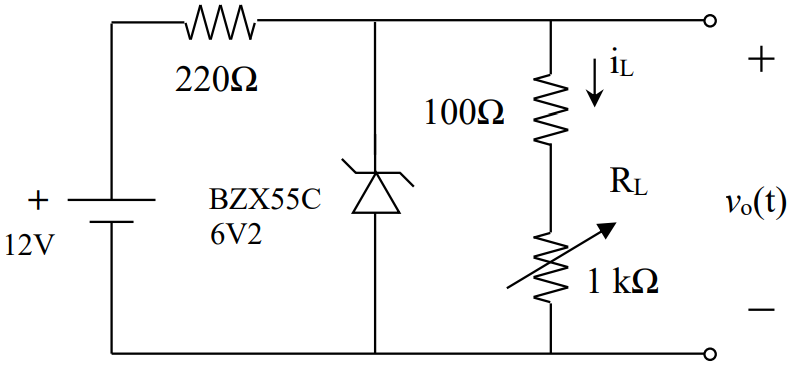
\includegraphics[width = 0.75\textwidth]{4_1.png}
    \caption{Circuit schematic for the step 4}
\end{figure} 
    
While we are changing potentiometer resistance from minimum to maximum (100 to 1000\(\Omega\)), the first output voltage has started to increase from 4V to 6V, and then, We observed a constant output voltage of 6V even as we continued to increase \(R_L\) resistance. From these results, we can conclude that the zener diode opens in reverse when the reverse bias voltage accross exceeds the \(-V_z\). Hence, zener diode has a regulation effect.
    
\section{Conclusion}

In conclusion, i-v characteristics of these AA119,BA159, BZX55C-6V2 diodes and half-wave rectifier circuit are investigated and the differences between these three diodes and zener diode are learned. Then it is observed that half-wave rectifier output same with the input signal where it is positive and equal to zero at input is negative. It was then observed that the clamping circuit gave an input signal which is clamped to zero and shifted below zero. Lastly, it is experimented that zener diode has an regulation effect. 



\section*{Appendix A}
\begin{itemize}
    \item PreLab Preprataion 6 hours
    \item Experimental Work 2  hours
    \item Report Writing 6 hours
\end{itemize}

\end{document}

%%%%%%%%%%%%%%%%%%%%%%   EXAMPLE TABLE   %%%%%%%%%%%%%%%%%%%%%%%%%%%%%%%%
\begin{table}[H]
\begin{center}
    \caption{Resistance reading by color code convention.}
    \vspace{2mm}
    \begin{tabular}{||c | c | c||} 
        \hline
        Color Order & Value & Tolerance \\ [0.5ex] 
        \hline\hline
        Brown / Black / Red / Gold & 1k\( \Omega \) & \( \% \) 5  \\ 
        \hline
        Yellow / Violet / Red / Gold & 4.7k\( \Omega \) & \( \% \) 5   \\
        \hline
        Brown / Grey / Orange / Gold & 18k\( \Omega \) & \( \% \) 5  \\ [1ex] 
        \hline
    \end{tabular}
\end{center}
\end{table}


%%%%%%%%%%%%%%%%%%%%%%   EXAMPLE IMAGE   %%%%%%%%%%%%%%%%%%%%%%%%%%%%%%%%
\begin{figure}[H]
\centering
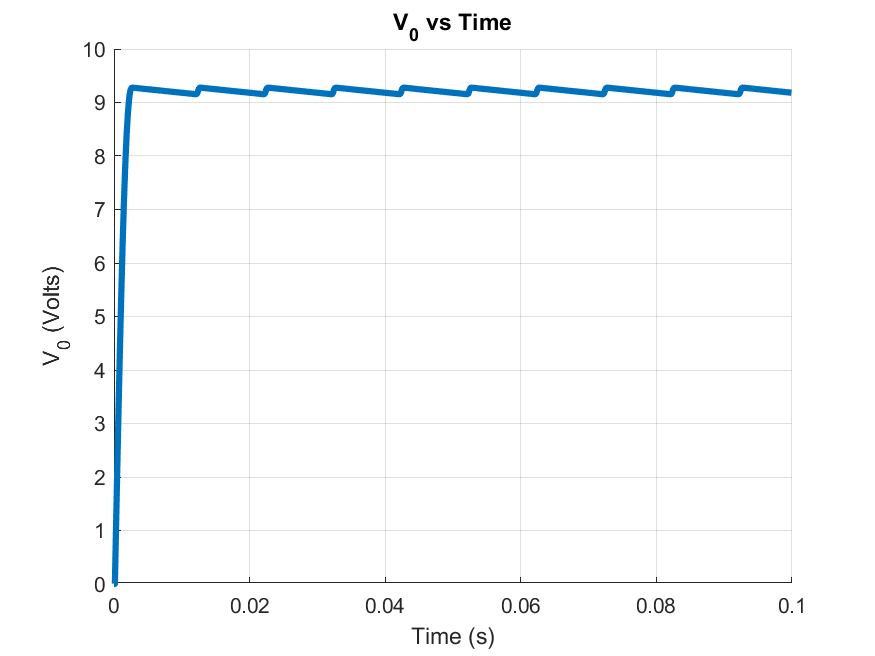
\includegraphics[width = 0.75\textwidth]{5.png}
\caption{Circuit schematic for the step 5}
\end{figure} 

%%%%%%%%%%%%%%%%%%%%%%   EXAMPLE IMAGE FROM PDF   %%%%%%%%%%%%%%%%%%%%%%%%%%%%%%%%
\begin{figure}[H] \centering{
	\includegraphics[scale=0.25]{2a_plot.pdf}}
	\caption{Experiment 2}
\end{figure}
	